
%=====================================================================
\section{Irrational rotation, Sturmian coding and non-periodicity}\label{sec:rotation}
%=====================================================================
Throughout this section $x_0\ge2$ is arbitrary, $T^*$ is the entry index of Lemma~\ref{lem:window}, and the \emph{tail} is the word $c=(c_j)_{j\ge0}$ with $c_j=1$ if the prime fired at step $T^*+j$ is $2$ and $c_j=0$ if it is $3$. Let $A=\ln18$, $B=\ln48$, $L=A+B=\ln864$ and $\theta=B/L$.

\subsection{The rotation}
\begin{lemma}[Irrationality]\label{lem:irr}
$\theta=\ln48/\ln864$ is irrational.
\end{lemma}
\begin{proof} If $\theta=r/s$ with $r,s\ge1$ then $48^s=864^r$, i.e. $2^{4s}3^s=2^{5r}3^{3r}$. Unique factorisation gives $4s=5r$ and $s=3r$, so $12r=5r$, which is impossible. \end{proof}
Put $z_j=(f_{T^*+j}+A)/L\in[0,1)$. This normalises the window $[-A,B)$ of length $L$ to $[0,1)$.
\begin{proposition}[Conjugacy to a rotation]\label{prop:rotation}
For all $j\ge0$: $c_j=1$ iff $z_j\ge1-\theta$, and
\[
z_{j+1}=\{z_j+\theta\}\quad(\text{fractional part}),\qquad\text{so}\quad z_j=\{z_0+j\theta\}.
\]
\end{proposition}
\begin{proof}
$2$ is fired iff $f>0$ iff $z>A/L=1-\theta$; since $f\ne0$ (Proposition~\ref{prop:twocounter}) the inequality is strict, and $z=1-\theta$ is excluded by Lemma~\ref{lem:window}(i) (it corresponds to $f=0$, which cannot occur), so equivalently $z\ge1-\theta$. If $2$ is fired, $f'=f-A$ gives $z'=z-A/L=z+\theta-1$, and $z+\theta\ge1$ so $z'=\{z+\theta\}$. If $3$ is fired, $f'=f+B$ gives $z'=z+\theta$ with $z<1-\theta$, so $z'=\{z+\theta\}$. \end{proof}
In words: the two valuation translations are one rotation of the circle $\R/L\Z$ by the angle $B\equiv-A$, and the fired prime is the code of the arc $[-A,0)\mapsto3$, $[0,B)\mapsto2$; the arc coded by $3$ has length $A=L-B$, equal to the rotation angle taken modulo $L$ (Figure~\ref{fig:rotation}).
\begin{figure}[ht]\centering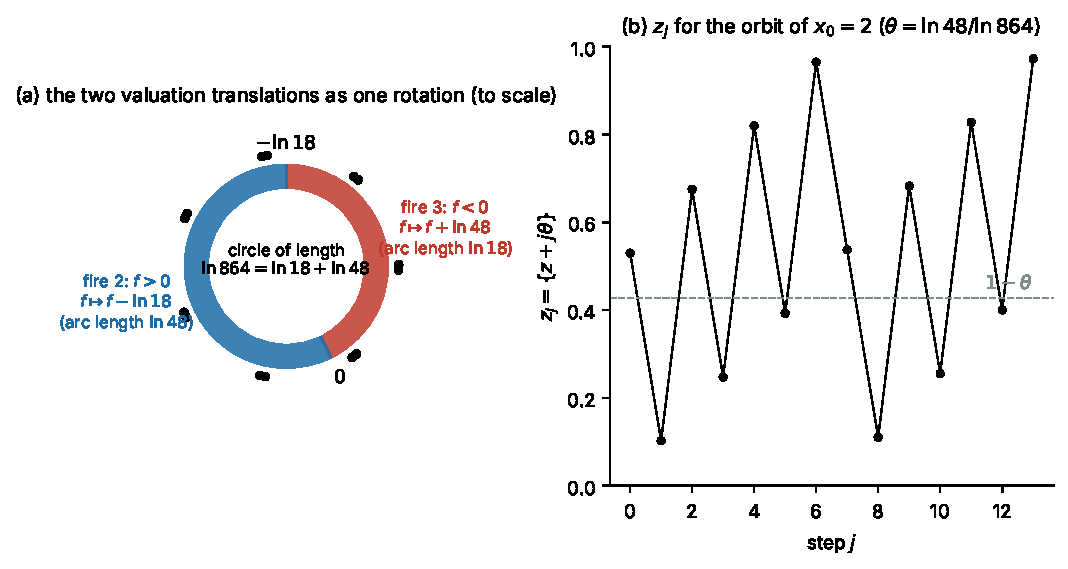
\includegraphics[width=.98\textwidth]{../figures/fig1_rotation.pdf}
\caption{(a) The circle of length $\ln864=\ln18+\ln48$ drawn to scale. Firing $2$ translates $f$ by $-\ln18$ on the blue arc $[0,\ln48)$, firing $3$ translates by $+\ln48$ on the red arc $[-\ln18,0)$; the dots are fourteen consecutive points of the orbit of $x_0=2$. (b) The same orbit in normalised coordinates $z_j=\{z_0+j\theta\}$.}\label{fig:rotation}\end{figure}

\begin{corollary}[Mechanical word]\label{cor:mech}
$c_j=\Fl z_0+(j+1)\theta\rfloor-\Fl z_0+j\theta\rfloor$ for all $j\ge0$.
\end{corollary}
\begin{proof} By Proposition~\ref{prop:rotation}, $c_j=1$ iff $z_j+\theta\ge1$ iff $\Fl z_j+\theta\rfloor=1$, so $c_j=\Fl z_j+\theta\rfloor$ with $z_j=z_0+j\theta-\Fl z_0+j\theta\rfloor$. Hence $c_j=\Fl z_0+(j+1)\theta\rfloor-\Fl z_0+j\theta\rfloor$. \end{proof}
Thus the tail is the mechanical word of slope $\theta$ and intercept $z_0$. Its structure is elementary.
\begin{proposition}[Blocks]\label{prop:blocks}
The tail contains no two consecutive $3$'s and no three consecutive $2$'s. Equivalently, between two consecutive $3$'s there are one or two $2$'s.
\end{proposition}
\begin{proof}
After firing $3$ from $f\in[-A,0)$ the new value is $f+B\ge B-A=\ln(8/3)>0$, so $2$ is fired next. After firing $2$ from $f\in(0,B)$ the value is $f-A<B-A=\ln(8/3)$; if it is positive $2$ may be fired once more, and then the value is $<\ln(8/3)-A<0$, so $3$ is fired. \end{proof}

\subsection{Non-periodicity}
\begin{theorem}[Non-periodicity]\label{thm:nonper}
For every $x_0\ge2$ the \textsf{MAXPP} itinerary is not eventually periodic.
\end{theorem}
\begin{proof}
Suppose it is periodic from some $n_0\ge T^*$ with period $q\ge1$, containing $a$ steps with prime $2$ and $b$ with prime $3$, $a+b=q$. After each period the valuation pair changes by the constant vector $(\Delta\alpha,\Delta\beta)=(-a+4b,\;2a-b)$ (Theorem~\ref{thm:A}), so $f$ changes by $\Delta\alpha\ln2-\Delta\beta\ln3$ per period. By Lemma~\ref{lem:window}, $f$ stays in the bounded window $[-A,B)$ for $n\ge T^*$, so this change per period is $0$. Since $\ln2/\ln3$ is irrational (unique factorisation), $\Delta\alpha=\Delta\beta=0$, i.e. $a=4b$ and $b=2a$, hence $a=b=0$, contradicting $q\ge1$. \end{proof}
\begin{remark}
Equivalently, by Corollary~\ref{cor:mech} the number of $2$'s in $n$ consecutive tail letters is $\Fl z+n\theta\rfloor$ up to a bounded term, and a period with $a$ twos in $q$ letters would force $\theta=a/q$, contradicting Lemma~\ref{lem:irr}; the two arguments are the same observation in different coordinates.
\end{remark}

\subsection{Factor complexity}
\begin{theorem}[Sturmian complexity]\label{thm:cx}
For every $x_0\ge2$ the tail word has $p(k)=k+1$ for every $k\ge1$. In particular its entropy is $0$.
\end{theorem}
\begin{proof}
\emph{Upper bound.} Write $\chi(y)=1$ if $\fp y\in[1-\theta,1)$ and $\chi(y)=0$ otherwise, so $c_j=\chi(z_0+j\theta)$. A factor of length $k$ starting at position $j$ is $\Psi_k(z_j)$ with
\[
\Psi_k(z)=\bigl(\chi(z),\chi(z+\theta),\dots,\chi(z+(k-1)\theta)\bigr).
\]
The function $z\mapsto\chi(z+i\theta)$ is constant on each half-open arc of $\R/\Z$ that contains none of its discontinuities, namely the points $z\equiv-i\theta$ (where $\fp{z+i\theta}=0$) and $z\equiv1-\theta-i\theta\equiv-(i+1)\theta$ (where $\fp{z+i\theta}=1-\theta$). For $0\le i\le k-1$ the discontinuities of all $k$ functions lie in $D_k=\{\fp{-i\theta}:0\le i\le k\}$. By Lemma~\ref{lem:irr} the $k+1$ points of $D_k$ are distinct, and they cut the circle into $k+1$ half-open arcs on each of which $\Psi_k$ is constant. Hence at most $k+1$ distinct factors of length $k$ occur.
\emph{Lower bound.} By Theorem~\ref{thm:nonper} the tail is not eventually periodic, so by the Morse--Hedlund lemma (Lemma~\ref{lem:mh}) $p(k)\ge k+1$ for every $k$. Combining, $p(k)=k+1$. Then $\ent=\lim\frac1k\ln(k+1)=0$ (Lemma~\ref{lem:entropy}). \end{proof}
A word with $p(k)=k+1$ for all $k$ is, by definition, a Sturmian word (one-sided, here in its tail).

\begin{theorem}[Autonomous Sturmian generation]\label{thm:B}
Let $x_0\ge2$ be arbitrary and let $(p_n)$ be the itinerary of \textsf{MAXPP}. Then:
\begin{enumerate}[label=(\roman*),itemsep=1pt]
\item $p_n\in\{2,3\}$ for all $n\ge T$ (Theorem~\ref{thm:A});
\item $(p_n)$ is not eventually periodic (Theorem~\ref{thm:nonper});
\item the tail after the entry index $T^*$ has factor complexity exactly $p(k)=k+1$ for every $k\ge1$, hence topological entropy $0$ (Theorem~\ref{thm:cx});
\item the selector is a function of the current integer alone, requires no external input and no memory, and the state $x_n$ is unbounded, $\log_2x_n\ge2n$.
\end{enumerate}
\end{theorem}
\noindent\emph{Source.} Items (i)--(iii) are Theorem GEN-4 of U4-GEN~\cite{u4gen}, whose complexity statement rests on the classical Sturmian theorem; the proofs here are self-contained (Appendix~\ref{app:classical}). Item (iv) makes quantitative the unbounded-state accounting of that theorem.
\begin{proof} (i)--(iii) are the cited theorems. For (iv), see Definition~\ref{def:maxpp} and Proposition~\ref{prop:growth} ($x_n\ge x_0\cdot4.5^n$ and $\log_24.5>2$). \end{proof}
Statement (ii) concerns all initial integers at once: unlike a statement about one designated orbit, it holds for every starting state $x_0\ge2$, because the proof uses only the prime-fire reduction, which is a property of arithmetic, and the irrationality of $\ln 2/\ln 3$ and of $\theta$.

\subsection{Continued fraction of the rotation number}
\begin{table}[ht]\centering\small
\begin{tabular}{@{}rrlr@{}}\toprule
$i$ & $a_i$ & convergent $p_i/q_i$ & $|q_i\theta-p_i|$\\\midrule
0 & 0 & 0/1 & $0.5725$ \\
1 & 1 & 1/1 & $0.4275$ \\
2 & 1 & 1/2 & $0.1451$ \\
3 & 2 & 3/5 & $0.1374$ \\
4 & 1 & 4/7 & $0.007708$ \\
5 & 17 & 71/124 & $0.006321$ \\
6 & 1 & 75/131 & $0.001386$ \\
7 & 4 & 371/648 & $0.0007753$ \\
8 & 1 & 446/779 & $0.0006112$ \\
9 & 1 & 817/1427 & $0.0001641$ \\
10 & 3 & 2897/5060 & $0.0001189$ \\
11 & 1 & 3714/6487 & $4.519e-5$ \\
12 & 2 & 10325/18034 & $2.852e-5$ \\
13 & 1 & 14039/24521 & $1.668e-5$ \\
\bottomrule\end{tabular}

\caption{Continued fraction expansion $\theta=[a_0;a_1,a_2,\dots]=[0;1,1,2,1,17,1,4,\dots]$ and convergents (computed to $60$ digits).}\label{tab:cf}\end{table}
Table~\ref{tab:cf} lists the first partial quotients. The large partial quotient $a_5=17$ means that the itinerary resembles a periodic word of period $7$ (four $2$'s and three $3$'s) over stretches of about a hundred steps before the defect $|7\theta-4|\approx0.0077$ accumulates; this is why finite prefixes of the itinerary can look periodic although the word is not (Figure~\ref{fig:itinerary}).
\begin{figure}[ht]\centering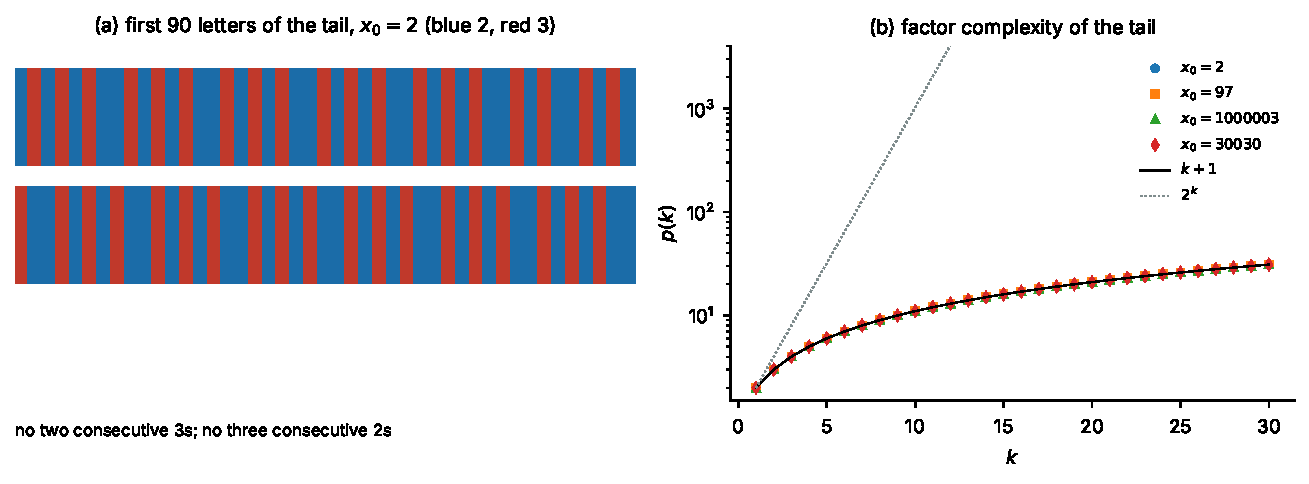
\includegraphics[width=.98\textwidth]{../figures/fig3_itinerary_complexity.pdf}
\caption{(a) The first $90$ letters of the tail for $x_0=2$. (b) Factor complexity $p(k)$ of the tail for four starts, $k\le30$ (computed): in every case $p(k)=k+1$ (Theorem~\ref{thm:cx}), against $2^k$.}\label{fig:itinerary}\end{figure}

%=====================================================================
\section{Exact frequencies, discrepancy and arithmetic growth}\label{sec:freq}
%=====================================================================
\begin{theorem}[Exact frequencies and growth]\label{thm:C}
Let $x_0\ge2$, $z=z_0$ and let $C_2(n)=\sum_{j<n}c_j$ be the number of $2$'s among the first $n$ letters of the tail. Then:
\begin{enumerate}[label=(\roman*),itemsep=1pt]
\item $C_2(n)=\Fl z+n\theta\rfloor$ for all $n\ge0$, hence $z-1<C_2(n)-n\theta\le z$ and $|C_2(n)-n\theta|<1$;
\item the frequency of $2$ is $\theta=\ln48/\ln864\approx0.572530$ and that of $3$ is $1-\theta=\ln18/\ln864\approx0.427470$;
\item $\log_2x_{T^*+n}=\log_2x_{T^*}+C_2(n)\log_2\tfrac92+(n-C_2(n))\log_2\tfrac{16}{3}$, and
\[
\lim_{n\to\infty}\frac{\log_2x_n}{n}=\theta\log_2\tfrac92+(1-\theta)\log_2\tfrac{16}3=2.2747033\ldots\text{ bits per step},
\]
with $\bigl|\log_2x_{T^*+n}-\log_2x_{T^*}-\rho n\bigr|<\log_2\tfrac{32}{27}<0.2452$ for the rate $\rho$ above.
\end{enumerate}
\end{theorem}
\noindent\emph{Source.} The exact frequencies, the discrepancy bound and the growth rate are recorded as GEN-5 in U4-GEN-C~\cite{u4genc}, a release that is not part of the commit-pinned collection~\cite{coll}; they are proved here.
\begin{proof}
(i) Summing Corollary~\ref{cor:mech} telescopes to $C_2(n)=\Fl z+n\theta\rfloor-\Fl z\rfloor=\Fl z+n\theta\rfloor$ since $z\in[0,1)$. Then $z+n\theta-1<C_2(n)\le z+n\theta$. (ii) follows from (i) and $0\le z<1$. (iii) Firing $2$ multiplies $x$ by $9/2$ and firing $3$ by $16/3$ (Proposition~\ref{prop:growth} with $N=2,3$), so the displayed identity holds. Put $a=\log_2\frac92$, $b=\log_2\frac{16}3$ and $C_2(n)=n\theta+\delta_n$ with $\delta_n\in(z-1,z]$ by (i). Then $C_2a+(n-C_2)b=n\rho+\delta_n(a-b)$ with $\rho=\theta a+(1-\theta)b$ and $a-b=\log_2\frac{27}{32}$. Thus $r_n=\log_2x_{T^*+n}-\log_2x_{T^*}-\rho n=\delta_n(a-b)$ lies in an interval of length $\log_2\frac{32}{27}$, and $r_0=0$ belongs to it; hence $|r_n|<\log_2\frac{32}{27}$, and $r_n/n\to0$. \end{proof}
The value $\ln48/\ln864=0.5725296677\ldots$ and the rate $2.27470332\ldots$ were confirmed numerically (Appendix~\ref{app:checks}, checks C5--C6).

\begin{corollary}[Beatty-type valuations]\label{cor:beatty}
For $n\ge0$, with $(\alpha_0,\beta_0)=(\alpha_{T^*},\beta_{T^*})$,
\[
\alpha_{T^*+n}=\alpha_0+4n-5\Fl z+n\theta\rfloor,\qquad
\beta_{T^*+n}=\beta_0-n+3\Fl z+n\theta\rfloor,\qquad
f_{T^*+n}=f_{T^*}+nB-L\Fl z+n\theta\rfloor.
\]
\end{corollary}
\begin{proof} Each $2$ contributes $(-1,+2)$ and each $3$ contributes $(+4,-1)$, so $\alpha_n=\alpha_0-C_2+4(n-C_2)=\alpha_0+4n-5C_2$ and $\beta_n=\beta_0+2C_2-(n-C_2)=\beta_0-n+3C_2$. Then $f_n=f_0+n(4\ln2+\ln3)-C_2(5\ln2+3\ln3)=f_0+nB-C_2L$ because $4\ln2+\ln3=\ln48$ and $5\ln2+3\ln3=\ln864$. \end{proof}
Thus the exponents of $2$ and $3$ in $x_n$ are Beatty-type sequences with slopes $4-5\theta$ and $3\theta-1$, both positive: numerically $4-5\theta=1.1373\ldots$ and $3\theta-1=0.7176\ldots$, so $x_n$ is divisible by roughly $2^{1.137n}3^{0.718n}$, and $\alpha_n\ln2-\beta_n\ln3=f_n$ stays bounded, as it must.

\begin{proposition}[Block frequencies]\label{prop:blockfreq}
Decompose the tail into the blocks $23$ and $223$ (Proposition~\ref{prop:blocks}); each block ends in a $3$. Both blocks occur with positive frequency, and the proportion of blocks equal to $223$ is
\[
\frac1{1-\theta}-2=\frac{\ln(8/3)}{\ln18}\approx0.3394.
\]
\end{proposition}
\begin{proof} By Theorem~\ref{thm:C}(i) the number of $3$'s among $n$ letters is $n(1-\theta)+O(1)$, so the number of blocks is the same and the average block length tends to $1/(1-\theta)=\ln864/\ln18=2.339\ldots\in(2,3)$. If a proportion $r$ of the blocks has length $3$ then $2(1-r)+3r=1/(1-\theta)$, so $r=1/(1-\theta)-2=\ln864/\ln18-2=\ln(864/324)/\ln18=\ln(8/3)/\ln18$. \end{proof}
\begin{figure}[ht]\centering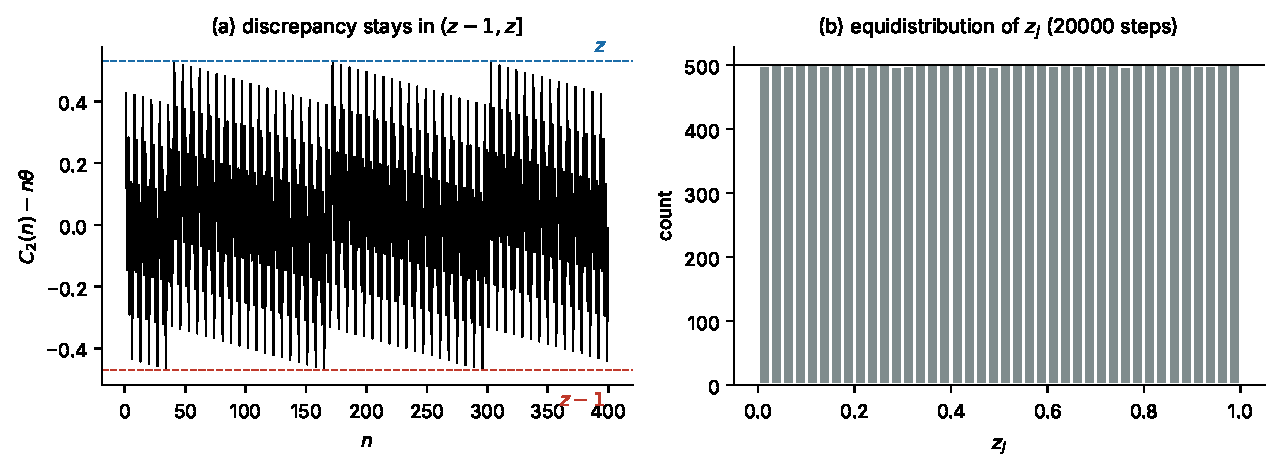
\includegraphics[width=.98\textwidth]{../figures/fig4_discrepancy.pdf}
\caption{(a) The discrepancy $C_2(n)-n\theta$ for $x_0=2$ stays in $(z-1,z]$ (Theorem~\ref{thm:C}). (b) The points $z_j$ equidistribute on $[0,1)$ (computed, $20000$ steps).}\label{fig:discrepancy}\end{figure}
\begin{figure}[ht]\centering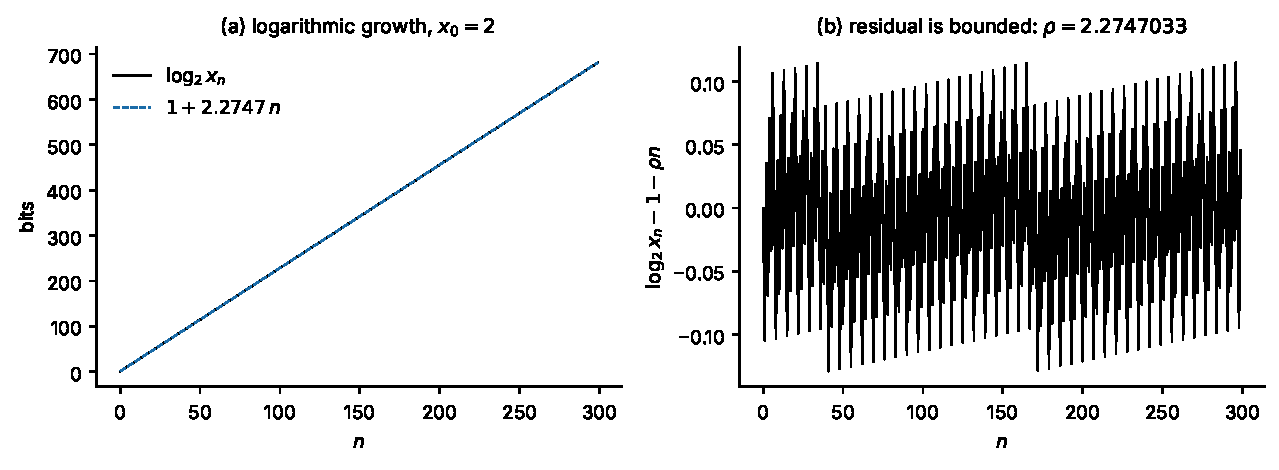
\includegraphics[width=.98\textwidth]{../figures/fig5_growth.pdf}
\caption{(a) $\log_2x_n$ for $x_0=2$ and the line $1+\rho n$ with $\rho=2.2747033$. (b) The residual stays within $\pm0.13$, inside the bound $\log_2\frac{32}{27}$ of Theorem~\ref{thm:C}(iii).}\label{fig:growth}\end{figure}

%=====================================================================
\section{Composite branches and renewal of prime support}\label{sec:composite}
%=====================================================================
Prime-fire selectors use only prime branch values. If $N$ may be composite, the valuation law of Theorem~\ref{thm:valuation} still applies, but the set of primes dividing $x$ is no longer controlled by Theorem~\ref{thm:A}. This section determines exactly when primes enter and leave the support and characterises the trajectories whose total support is finite.

\subsection{Entry and exit of primes}
Write $\supp(x)$ for the set of primes dividing $x$.
\begin{lemma}[Renewal]\label{lem:renewal}
Let $N\mid x$, $N\ge2$, $x'=T_N(x)$ and let $q$ be a prime.
\begin{enumerate}[label=(\roman*),itemsep=1pt]
\item \emph{(Entry)} $q\notin\supp(x)$ and $q\in\supp(x')$ iff $q\mid N+1$ and $q\nmid x$.
\item \emph{(Exit)} $q\in\supp(x)$ and $q\notin\supp(x')$ iff $v_q(N)=v_q(x)$ and $q\nmid N+1$.
\item In particular $\supp(x')\subset\supp(x)\cup\supp(N+1)$, and $\supp(N)\subset\supp(x)$.
\end{enumerate}
\end{lemma}
\begin{proof}
By Theorem~\ref{thm:valuation}, $v_q(x')=v_q(x)+2v_q(N+1)-v_q(N)$, and $v_q(x)-v_q(N)\ge0$ by legality, so
\[
v_q(x')=\underbrace{\bigl(v_q(x)-v_q(N)\bigr)}_{\ge0}+\underbrace{2v_q(N+1)}_{\ge0}.
\]
(i) If $q\nmid x$ then $q\nmid N$ (as $N\mid x$), so $v_q(x')=2v_q(N+1)$, which is positive iff $q\mid N+1$. (ii) $v_q(x')=0$ iff both summands vanish, i.e. $v_q(N)=v_q(x)$ and $q\nmid N+1$. (iii) follows from the displayed identity. \end{proof}
Entry therefore requires only that $q$ divides $N+1$; exit requires that $N$ exhausts the full power of $q$ in $x$ \emph{and} that $q$ does not divide $N+1$. Note that $q\mid N$ and $q\mid N+1$ cannot hold together, so a prime that divides $N$ either stays (if $v_q(N)<v_q(x)$) or leaves.

For a trajectory $(x_n)$ with branch values $(N_n)$ define the \emph{total prime support} $\mathcal S=\bigcup_{n\ge0}\supp(x_n)$.

\subsection{Finite support if and only if finitely many branches}
\begin{theorem}[Størmer, imported]\label{thm:stormer}
For every finite set $P$ of primes there are only finitely many pairs of consecutive positive integers $(m,m+1)$ both of whose prime factors lie in $P$.
\end{theorem}
This is Størmer's theorem (1897); it is quoted without proof. Table~\ref{tab:stormer} lists the branch values $N\ge2$ with both $N$ and $N+1$ $P$-smooth for the first four prime sets (computed by exhaustive search among $P$-smooth integers up to $10^{13}$, resp.\ $10^{12}$; the search bound is consistent with Størmer's bounds but is not itself a proof).
\begin{table}[ht]\centering\small
\begin{tabular}{@{}lrrp{0.5\textwidth}@{}}\toprule
$S$ & $\#\{N\ge2\}$ & $\max N$ & smallest values of $N$ with $N,N+1$ both $S$-smooth\\\midrule
$\{2,3\}$ & 3 & 8 & 2, 3, 8 \\
$\{2,3,5\}$ & 9 & 80 & 2, 3, 4, 5, 8, 9, 15, 24, 80 \\
$\{2,3,5,7\}$ & 22 & 4374 & 2, 3, 4, 5, 6, 7, 8, 9, 14, 15, \dots \\
$\{2,3,5,7,11\}$ & 39 & 9800 & 2, 3, 4, 5, 6, 7, 8, 9, 10, 11, \dots \\
\bottomrule\end{tabular}

\caption{Branch values $N\ge2$ such that $N$ and $N+1$ both have all prime factors in $P$ (computed).}\label{tab:stormer}\end{table}

\begin{theorem}[Support renewal]\label{thm:D}
Let $x_0\ge2$ and let $(N_n)$ be any legal sequence of branch values. Then the total prime support $\mathcal S$ is finite if and only if $\{N_n:n\ge0\}$ is finite.
\end{theorem}
\noindent\emph{Source.} The valuation-update and renewal lemmas and Proposition~S of U4-GEN-C~\cite{u4genc}, a release that is not part of the collection~\cite{coll}, state this equivalence; Størmer's theorem is imported. The proof given here is self-contained.
\begin{proof}
($\Leftarrow$) If the branch values lie in a finite set $\mathcal N$, Lemma~\ref{lem:renewal}(iii) gives inductively $\supp(x_n)\subset\supp(x_0)\cup\bigcup_{N\in\mathcal N}\supp(N+1)$ for all $n$, a finite set.

($\Rightarrow$) Let $\mathcal S$ be finite. For each $n$, every prime factor of $N_n$ divides $x_n$ (since $N_n\mid x_n$), and every prime factor $q$ of $N_n+1$ divides $x_{n+1}$, because $v_q(x_{n+1})\ge2v_q(N_n+1)>0$ by the displayed identity in the proof of Lemma~\ref{lem:renewal}. So both $N_n$ and $N_n+1$ are $\mathcal S$-smooth. By Theorem~\ref{thm:stormer} only finitely many $N$ have this property. \end{proof}

\begin{corollary}[Prime-fire selectors never renew]\label{cor:norenewal}
For every prime-fire selector and every $x_0\ge2$ the total support is contained in the primes $\le\max(3,P^+(x_0))$, where $P^+$ is the largest prime factor; in particular it is finite.
\end{corollary}
\begin{proof} A fire of $p$ introduces only primes dividing $p+1$, all of which are $<p$ for $p\ge5$ and $\le3$ for $p\in\{2,3\}$ (Lemma~\ref{lem:pplus1}). Induct on $n$. \end{proof}
Together with Theorem~\ref{thm:D} this says that the interesting behaviour of a selector with \emph{unboundedly many distinct} branch values is accompanied by genuine renewal of the prime support, and conversely a selector that keeps the support finite must reuse finitely many branches. Selectors with finite branch sets are the setting of Section~\ref{sec:complexity}, where an additional hypothesis on the guards is imposed.

\subsection{An example of renewal}
Consider the \emph{logarithmic-cap} rule: $N_n$ is the largest divisor of $x_n$ with $2\le N_n\le\lceil\log_2(x_n+1)\rceil$ (the bit length of $x_n$), and the smallest prime factor of $x_n$ if no such divisor exists. It is autonomous. Starting from $x_0=41,42,43$, $300$ steps (computed with exact integer exponents) produced $300$ distinct branch values in each of the three runs, a final support of $150$, $135$, $142$ primes respectively (about half the number of steps) and a cumulative support of $160$, $151$, $156$ primes, with $N_{\max}=2944$, $2935$, $2942$. By contrast \textsf{MAXPP} from $x_0=41$ uses $4$ branch values (the primes $41,2,3,7$) and a total support of $4$ primes over $3000$ steps. These are finite observations; they do not establish that the log-cap rule uses infinitely many branch values. They are consistent with Theorem~\ref{thm:D}, which relates the two phenomena: in the observed runs the number of distinct branch values and the size of the support grow together, while for \textsf{MAXPP} both stay bounded.
\begin{figure}[ht]\centering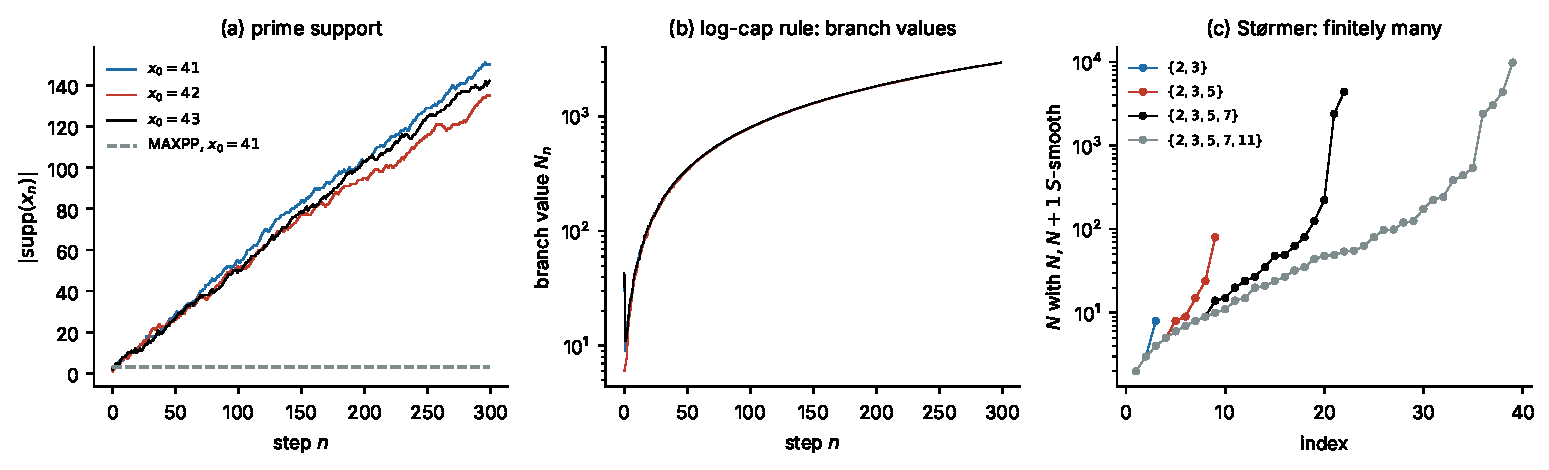
\includegraphics[width=.98\textwidth]{../figures/fig6_renewal.pdf}
\caption{(a) Size of the prime support $|\supp(x_n)|$ for the logarithmic-cap rule (three starts) and for \textsf{MAXPP} from $x_0=41$; (b) the branch values $N_n$ of the logarithmic-cap rule (logarithmic scale); (c) the branch values $N\ge2$ with $N,N+1$ both $S$-smooth for four prime sets $S$ (Størmer; finite in each case). All computed.}\label{fig:renewal}\end{figure}
